\section{Puzzle}
\subsection{} % 1
\begin{center}
    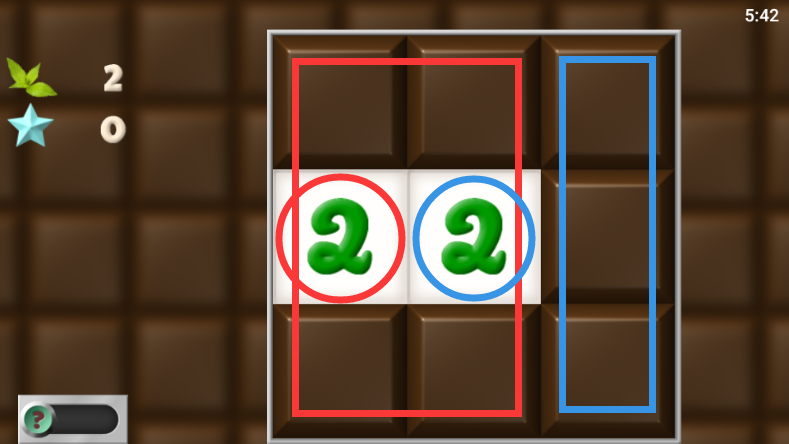
\includegraphics[width=0.7\textwidth]{puzzle/1-1.png}
\end{center}
因为红圈2,红框内有两个雷;又因为蓝圈2,蓝框内安全。
\begin{center}
    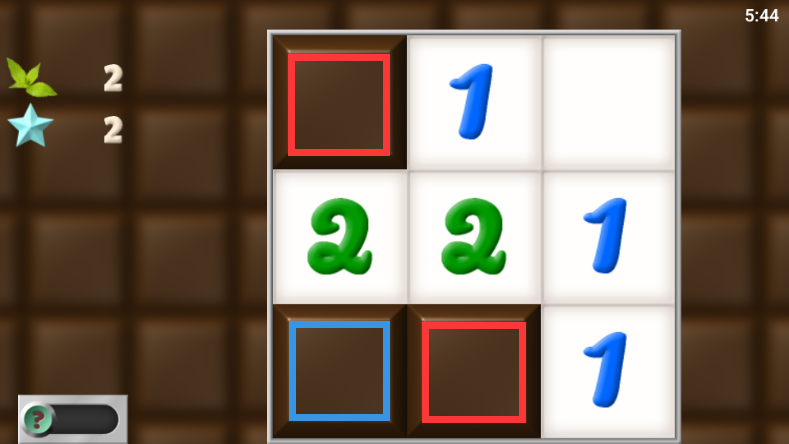
\includegraphics[width=0.7\textwidth]{puzzle/1-2.png}
\end{center}
数数,红框为雷,蓝框安全。

\subsection{} % 2
\begin{center}
    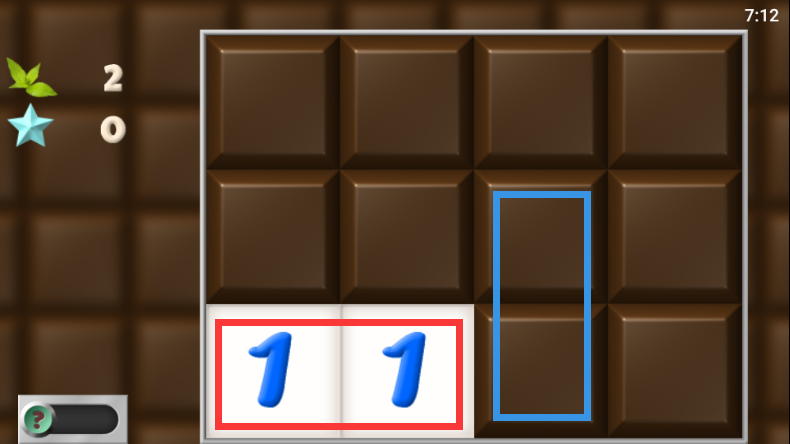
\includegraphics[width=0.7\textwidth]{puzzle/2-1.png}
\end{center}
红框11减法,蓝框安全。
\begin{center}
    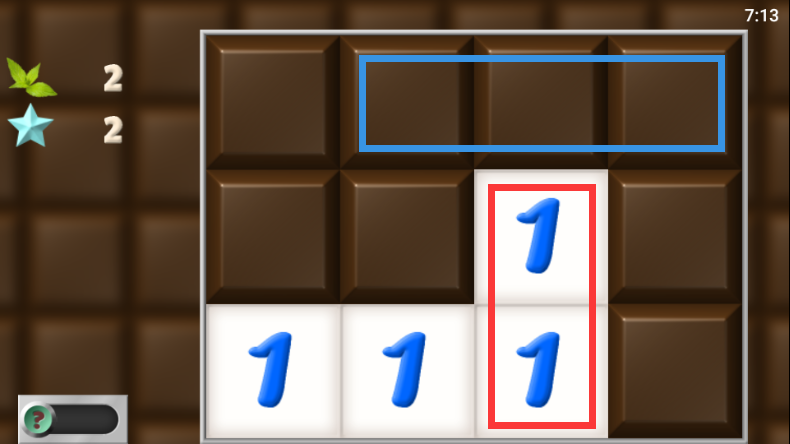
\includegraphics[width=0.7\textwidth]{puzzle/2-2.png}
\end{center}
红框11减法,蓝框安全。
\begin{center}
    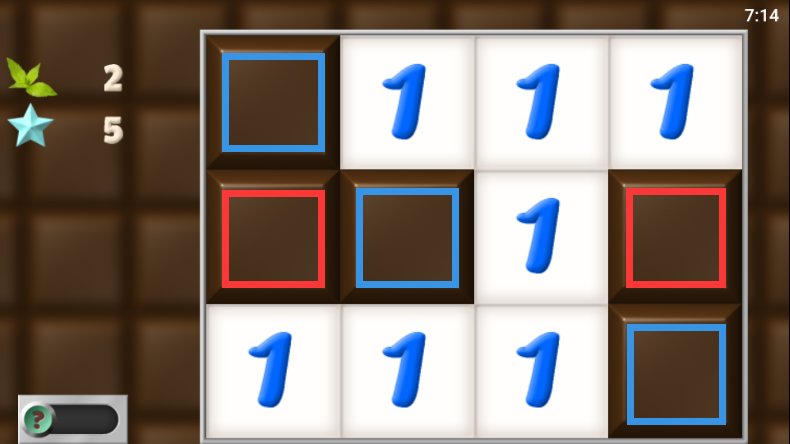
\includegraphics[width=0.7\textwidth]{puzzle/2-3.png}
\end{center}
数数,红框为雷,蓝框安全。

\subsection{} % 3
\begin{center}
    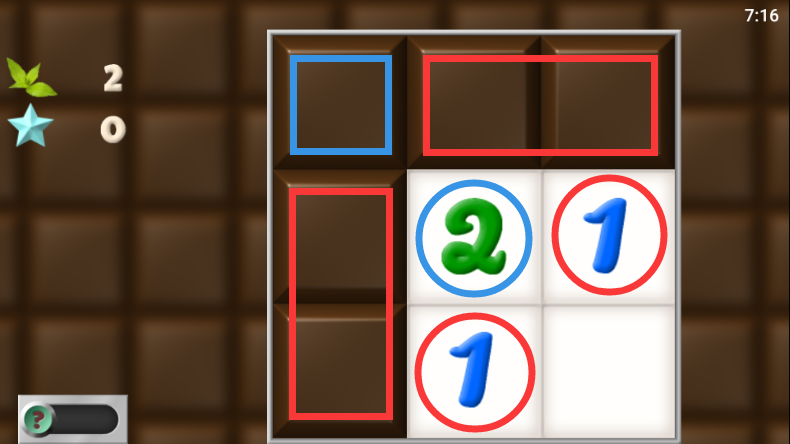
\includegraphics[width=0.7\textwidth]{puzzle/3-1.png}
\end{center}
由两个红圈1,两个红框各1雷;又因为蓝圈2,蓝框安全。
\begin{center}
    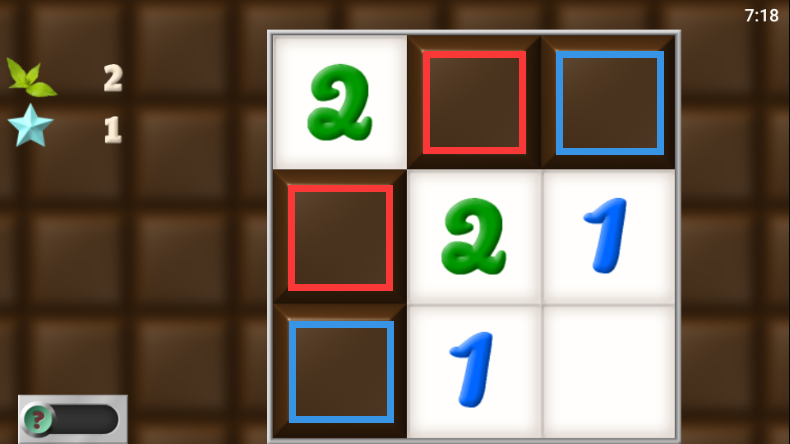
\includegraphics[width=0.7\textwidth]{puzzle/3-2.png}
\end{center}
数数,红框为雷,蓝框安全。

\subsection{} % 4
\begin{center}
    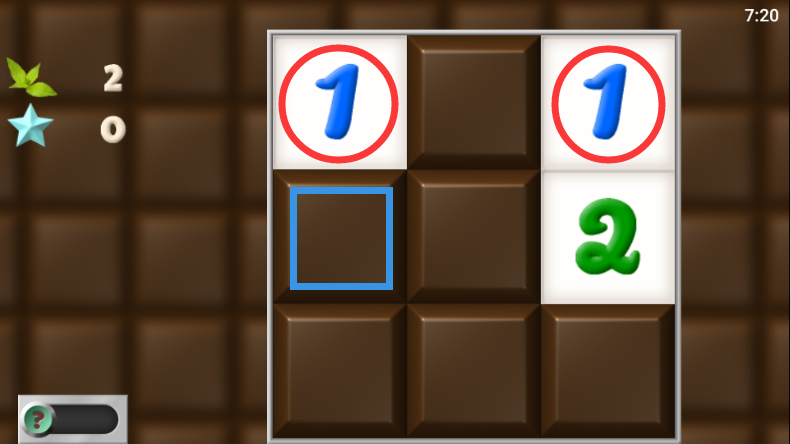
\includegraphics[width=0.7\textwidth]{puzzle/4-1.png}
\end{center}
红圈11减法,蓝框安全。
\begin{center}
    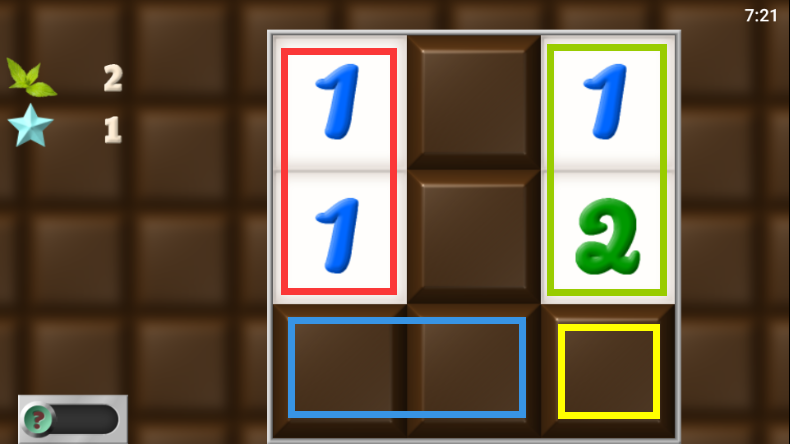
\includegraphics[width=0.7\textwidth]{puzzle/4-2.png}
\end{center}
红框11减法,蓝框安全。再用绿框12减法,黄框为雷。
\begin{center}
    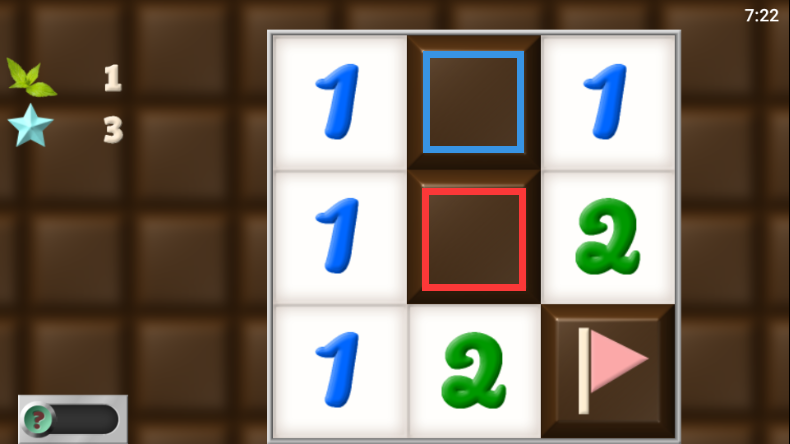
\includegraphics[width=0.7\textwidth]{puzzle/4-3.png}
\end{center}
数数,红框为雷,蓝框安全。

\subsection{} % 5
\begin{center}
    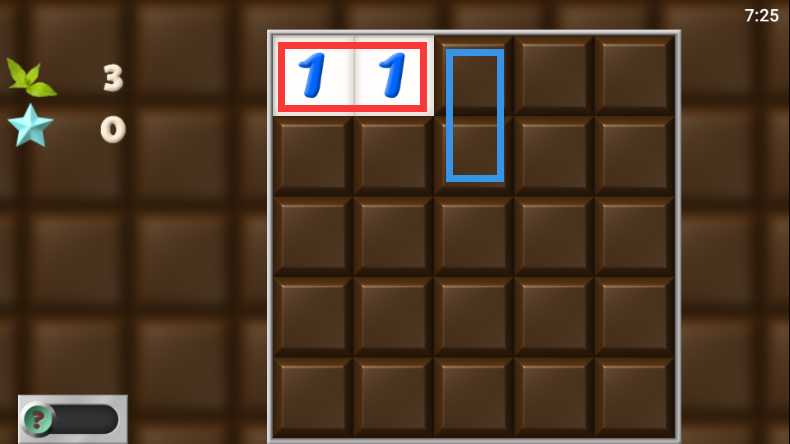
\includegraphics[width=0.7\textwidth]{puzzle/5-1.png}
\end{center}
红框11减法,蓝框安全。
\begin{center}
    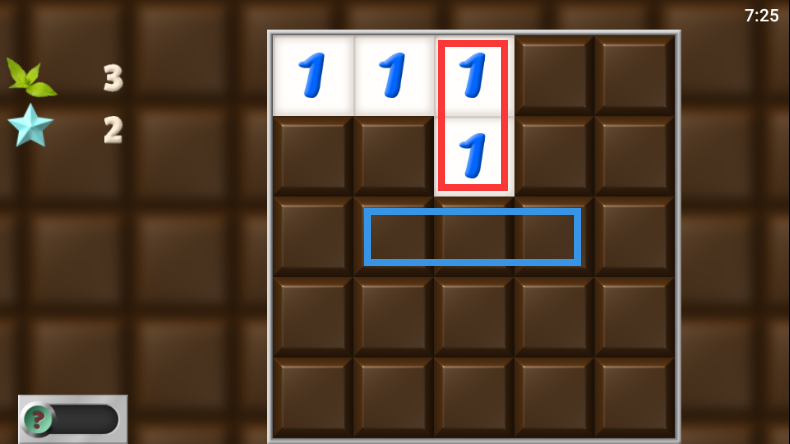
\includegraphics[width=0.7\textwidth]{puzzle/5-2.png}
\end{center}
红框11减法,蓝框安全。
\begin{center}
    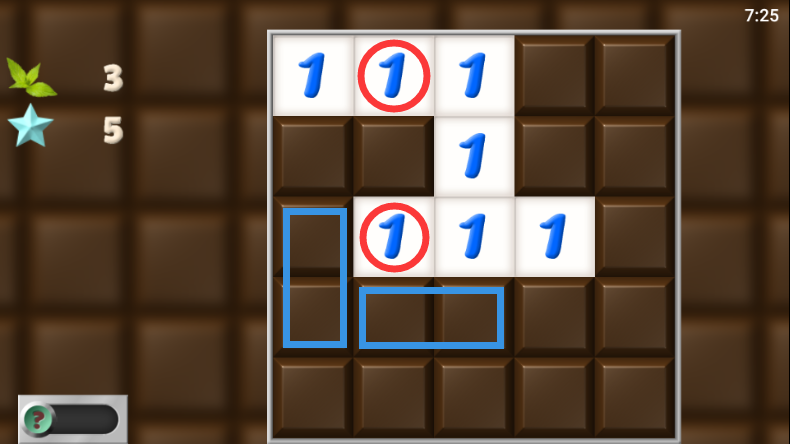
\includegraphics[width=0.7\textwidth]{puzzle/5-3.png}
\end{center}
红圈11减法,蓝框安全。
\begin{center}
    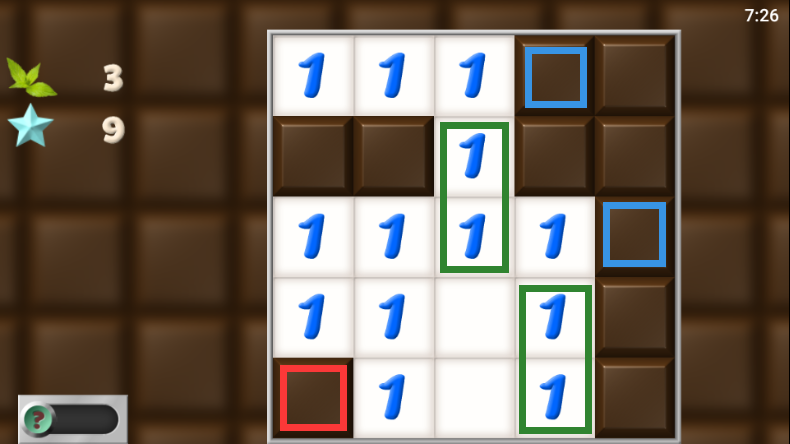
\includegraphics[width=0.7\textwidth]{puzzle/5-4.png}
\end{center}
数数,红框为雷。再分别用绿框11减法,两个蓝框安全。
\begin{center}
    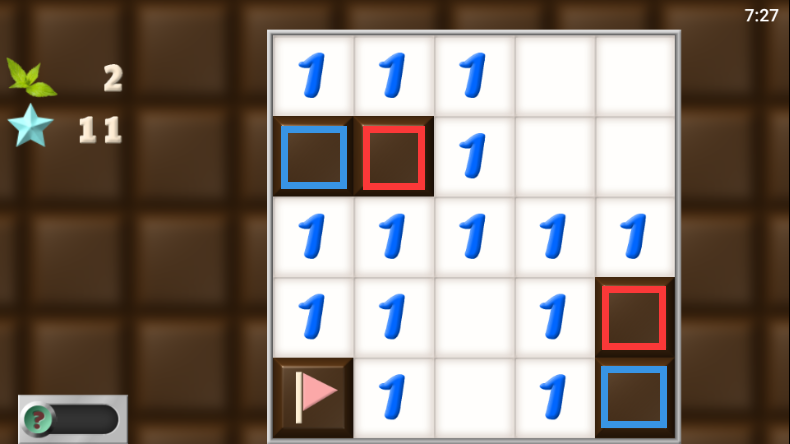
\includegraphics[width=0.7\textwidth]{puzzle/5-5.png}
\end{center}
数数,红框为雷,蓝框安全。

\subsection{} % 6
\begin{center}
    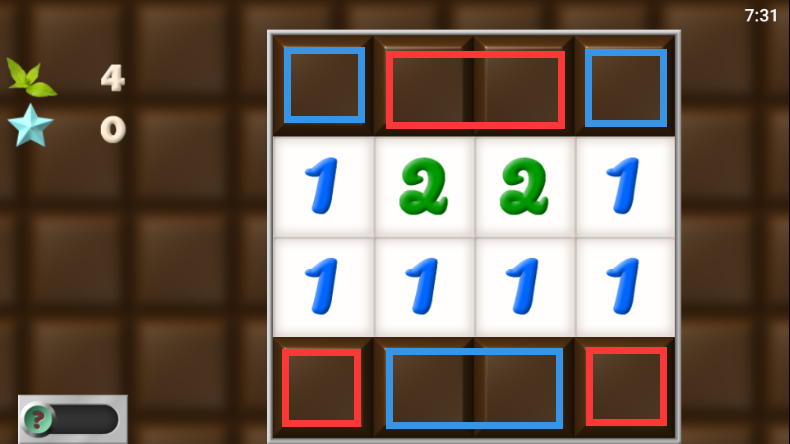
\includegraphics[width=0.7\textwidth]{puzzle/6-1.png}
\end{center}
上下分别用1221定式和1111定式,红框为雷,蓝框安全。

\subsection{} % 7
\begin{center}
    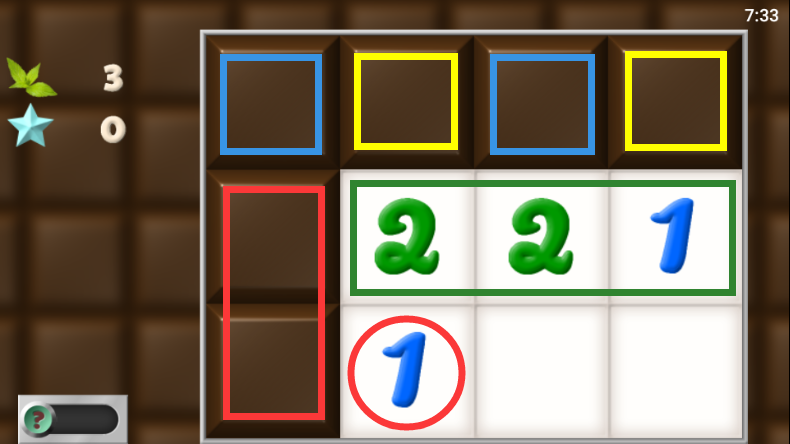
\includegraphics[width=0.7\textwidth]{puzzle/7-1.png}
\end{center}
由红圈1,红框有1雷;然后绿框形成121定式,黄框为雷,蓝框安全。

\subsection{} % 8
\begin{center}
    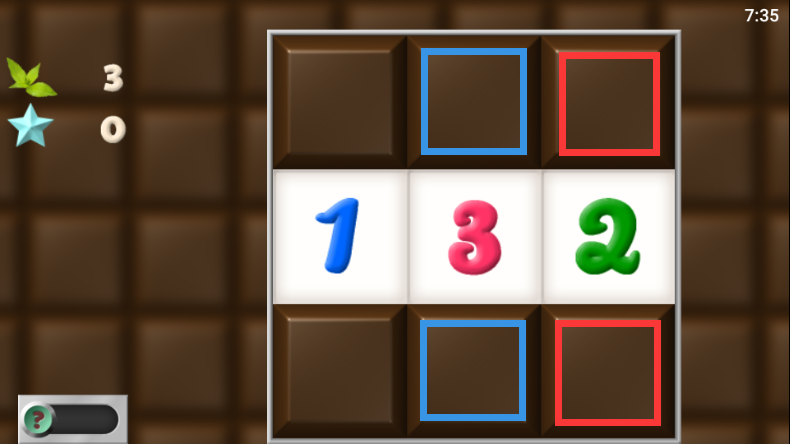
\includegraphics[width=0.7\textwidth]{puzzle/8-1.png}
\end{center}
由132定式,红框为雷,蓝框安全。

\subsection{} % 9
\begin{center}
    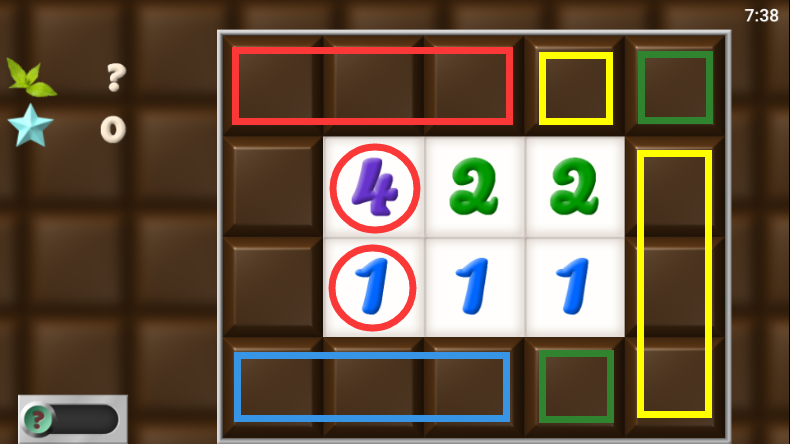
\includegraphics[width=0.7\textwidth]{puzzle/9-1.png}
\end{center}
红圈14减法,红框为雷,蓝框安全。然后数数,绿框为雷,黄框安全。
\begin{center}
    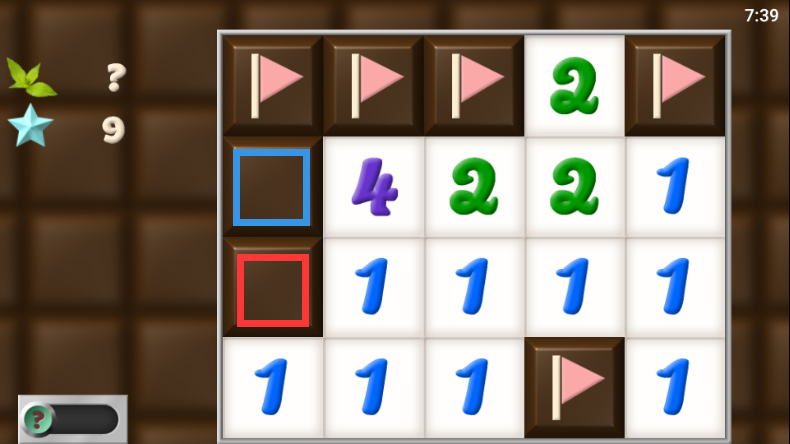
\includegraphics[width=0.7\textwidth]{puzzle/9-2.png}
\end{center}
数数,红框为雷,蓝框安全。

\subsection{} % 10
\begin{center}
    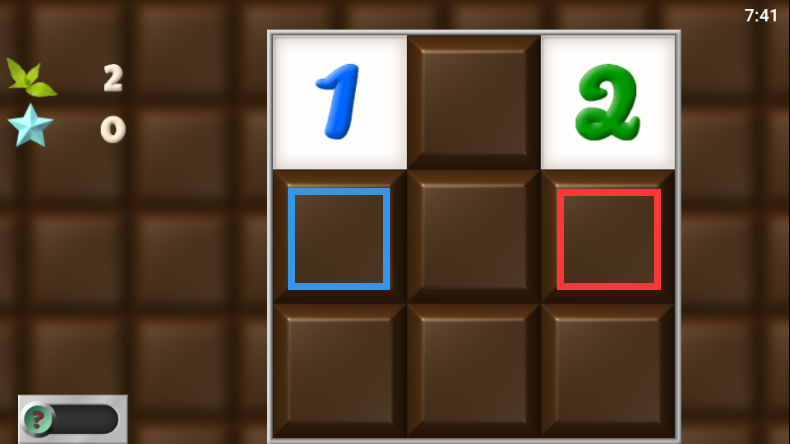
\includegraphics[width=0.7\textwidth]{puzzle/10-1.png}
\end{center}
12减法,红框为雷,蓝框安全。
\begin{center}
    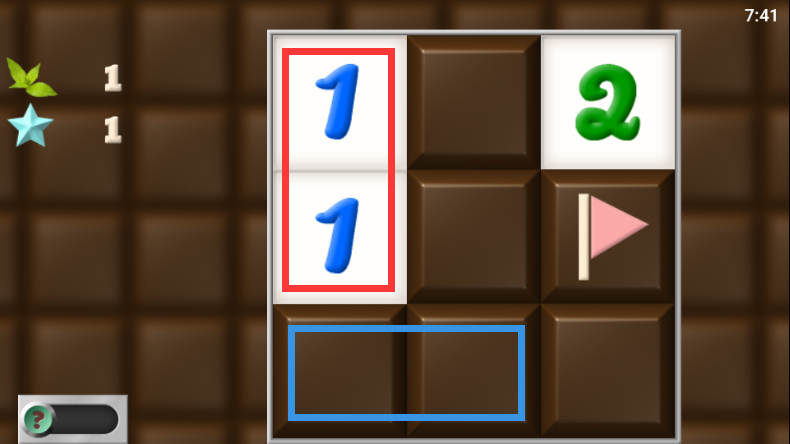
\includegraphics[width=0.7\textwidth]{puzzle/10-2.png}
\end{center}
红框11减法,蓝框安全。
\begin{center}
    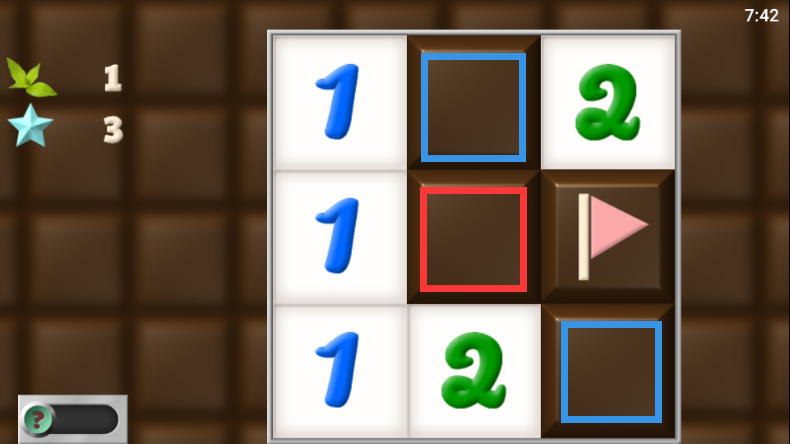
\includegraphics[width=0.7\textwidth]{puzzle/10-3.png}
\end{center}
数数,红框为雷,蓝框安全。

\subsection{} % 11
\begin{center}
    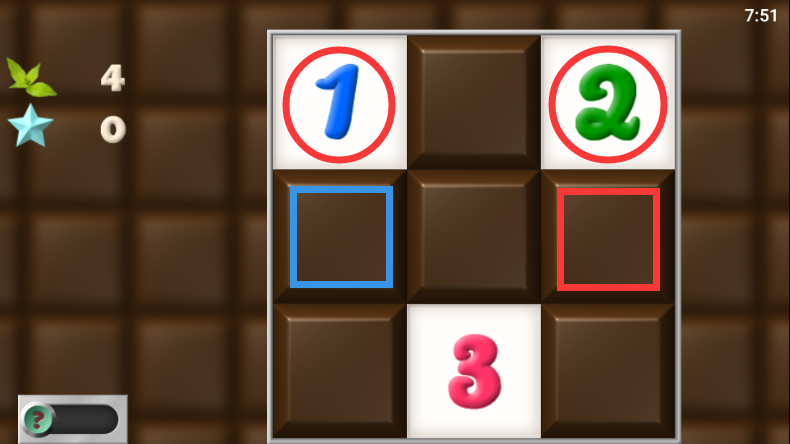
\includegraphics[width=0.7\textwidth]{puzzle/11-1.png}
\end{center}
红圈12减法,红框为雷,蓝框安全。
\begin{center}
    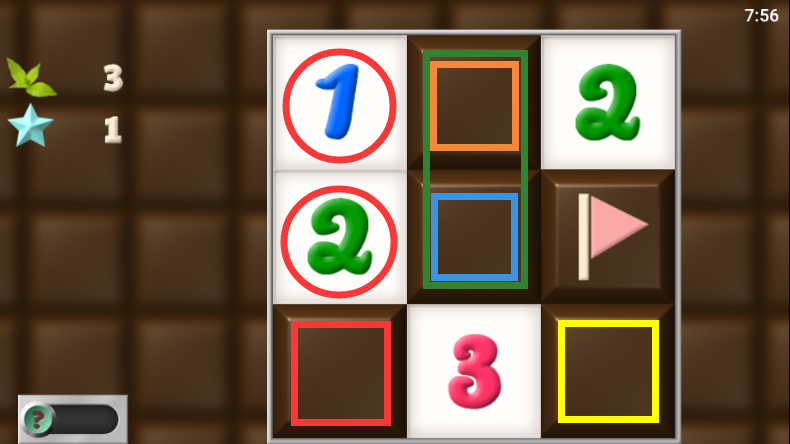
\includegraphics[width=0.7\textwidth]{puzzle/11-2.png}
\end{center}
红圈12减法,红框为雷,绿框有1雷;再数雷,排除绿框1雷,得黄框为雷。数数,橙框为雷,蓝框安全。

\subsection{} % 12
\begin{center}
    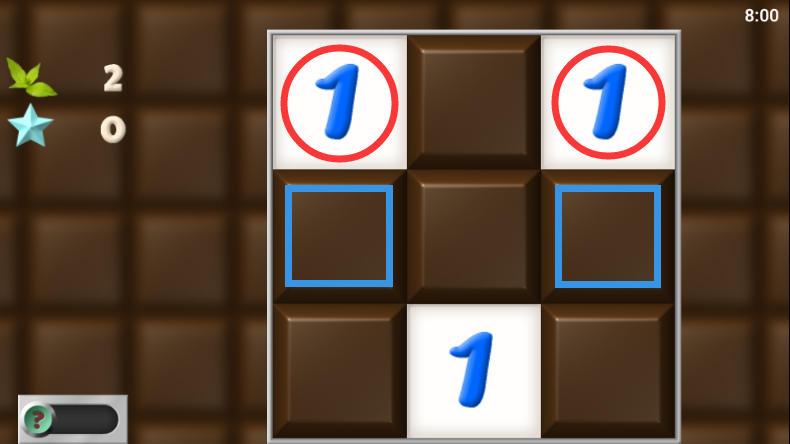
\includegraphics[width=0.7\textwidth]{puzzle/12-1.png}
\end{center}
红圈11减法得两个蓝框相等,又因为剩下一个1,两个蓝框均安全。
\begin{center}
    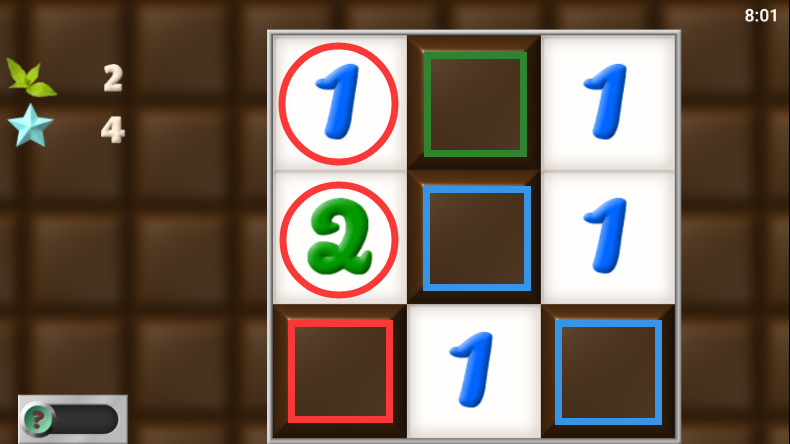
\includegraphics[width=0.7\textwidth]{puzzle/12-2.png}
\end{center}
红圈12减法,红框为雷。数数,绿框为雷,蓝框安全。

\subsection{} % 13
\begin{center}
    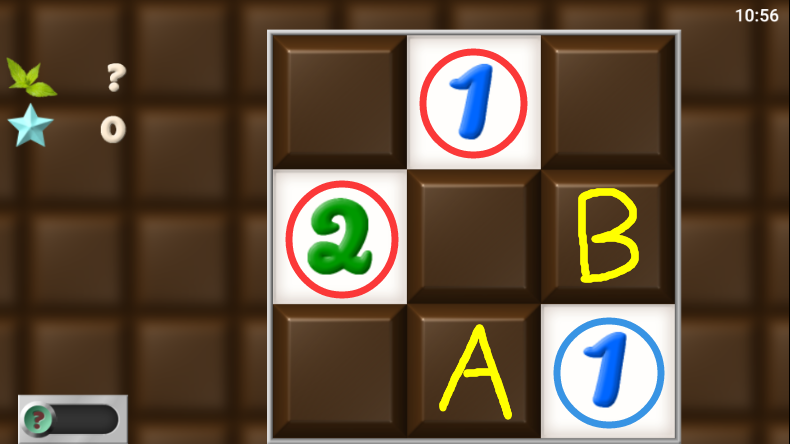
\includegraphics[width=0.7\textwidth]{puzzle/13-1.png}
\end{center}
红圈12减法得$A\ge B$,又因为蓝圈1,$B$安全。
\begin{center}
    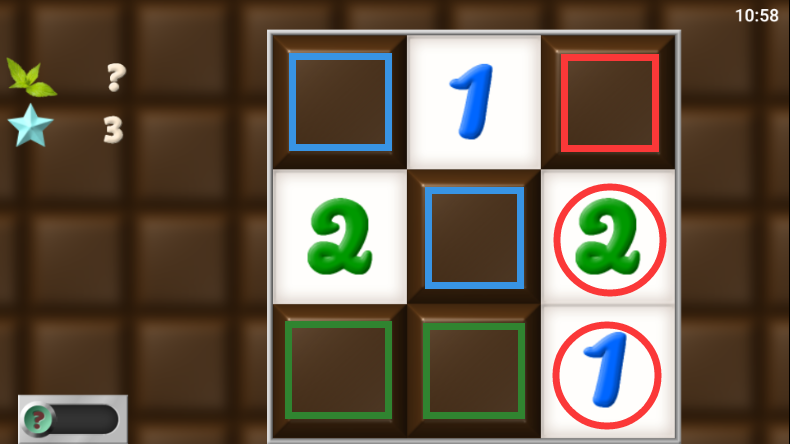
\includegraphics[width=0.7\textwidth]{puzzle/13-2.png}
\end{center}
红圈12减法,红框为雷。数数,绿框为雷,蓝框安全。

\subsection{} % 14
\begin{center}
    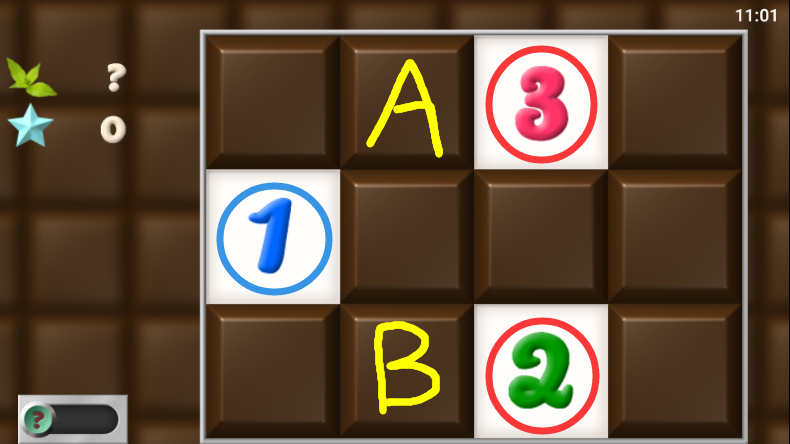
\includegraphics[width=0.7\textwidth]{puzzle/14-1.png}
\end{center}
红圈23减法得$A\ge B$,又因为蓝圈1,$B$安全。
\begin{center}
    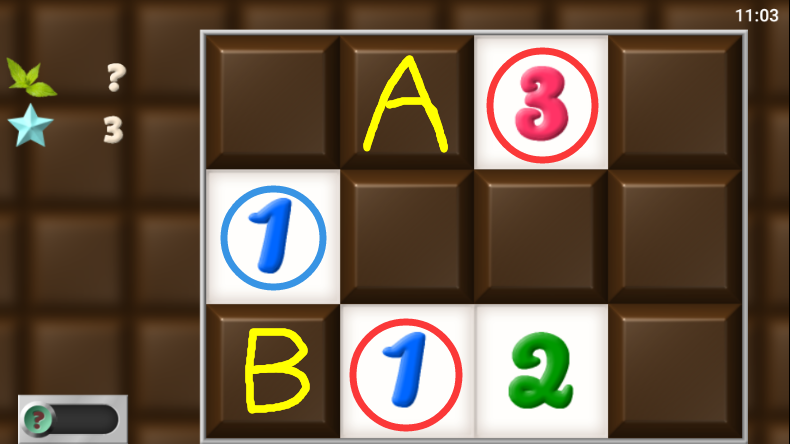
\includegraphics[width=0.7\textwidth]{puzzle/14-2.png}
\end{center}
红圈13减法得$A\ge B$,又因为蓝圈1,$B$安全。
\begin{center}
    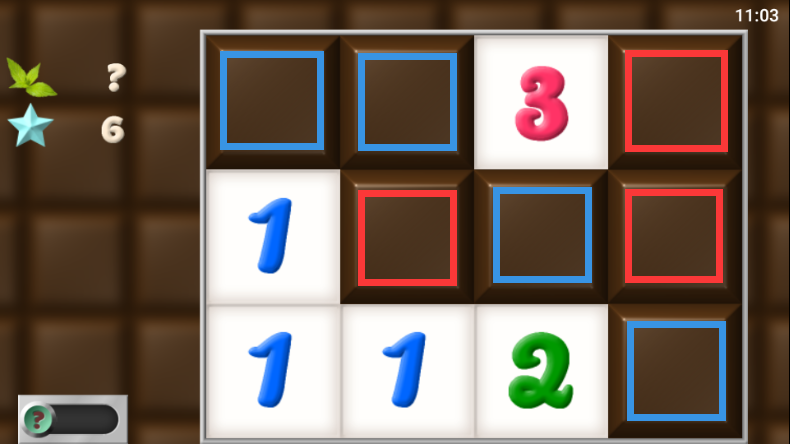
\includegraphics[width=0.7\textwidth]{puzzle/14-3.png}
\end{center}
数数,红框为雷,蓝框安全。

\subsection{} % 15
\begin{center}
    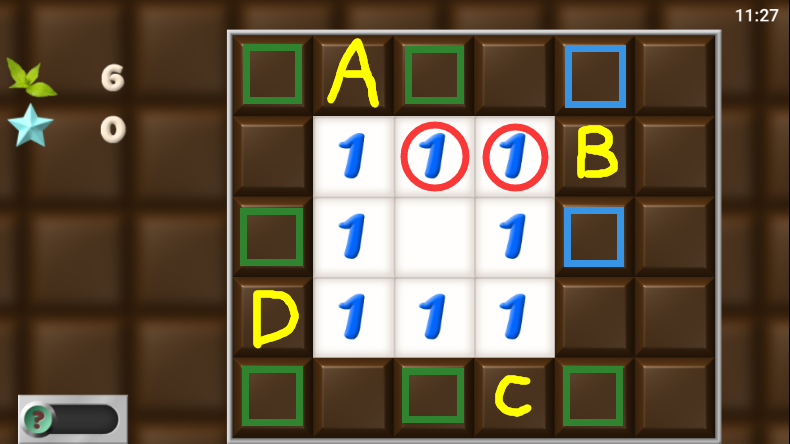
\includegraphics[width=0.7\textwidth]{puzzle/15-1.png}
\end{center}
红圈11减法得$A\ge B$,同理$B\ge C$,$C\ge D$,$D\ge A$;所以$A=B=C=D$。考虑$A=B$,再用红圈11做减法得到蓝框安全,同理绿框安全。
\begin{center}
    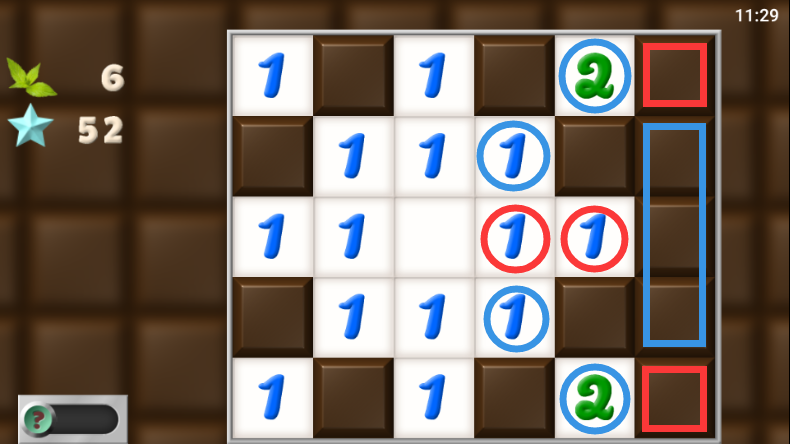
\includegraphics[width=0.7\textwidth]{puzzle/15-2.png}
\end{center}
红圈11减法得蓝框安全。再分别用两个蓝圈12减法得红框为雷。
\begin{center}
    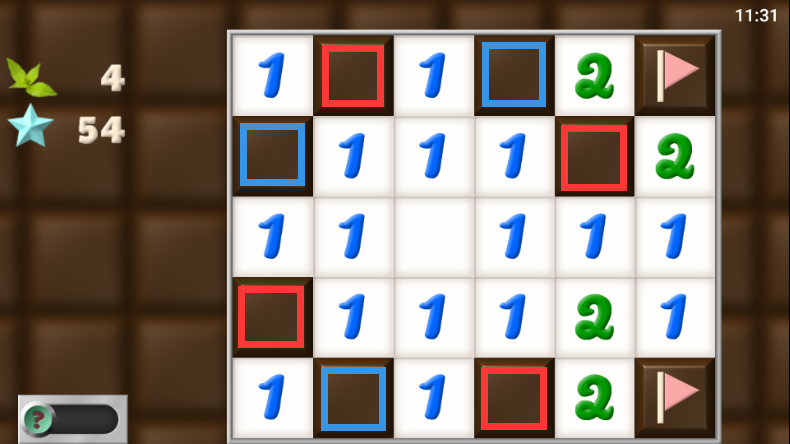
\includegraphics[width=0.7\textwidth]{puzzle/15-3.png}
\end{center}
数数,红框为雷,蓝框安全。

\subsection{} % 16
\begin{center}
    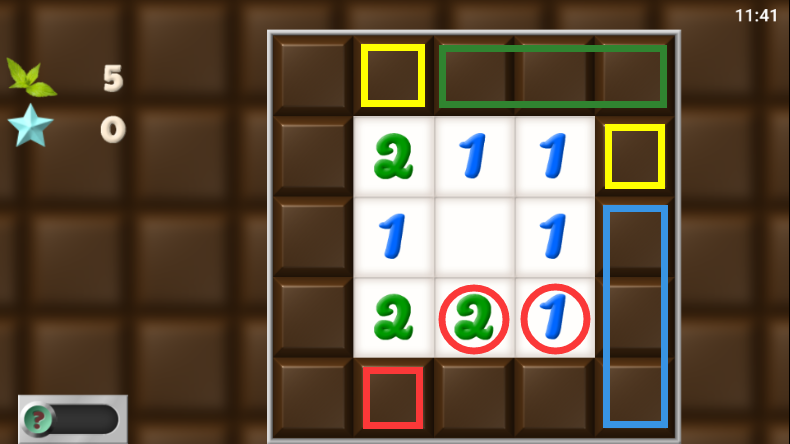
\includegraphics[width=0.7\textwidth]{puzzle/16-1.png}
\end{center}
红圈12减法得红框为雷,蓝框安全。数数,黄框为雷,绿框安全。
\begin{center}
    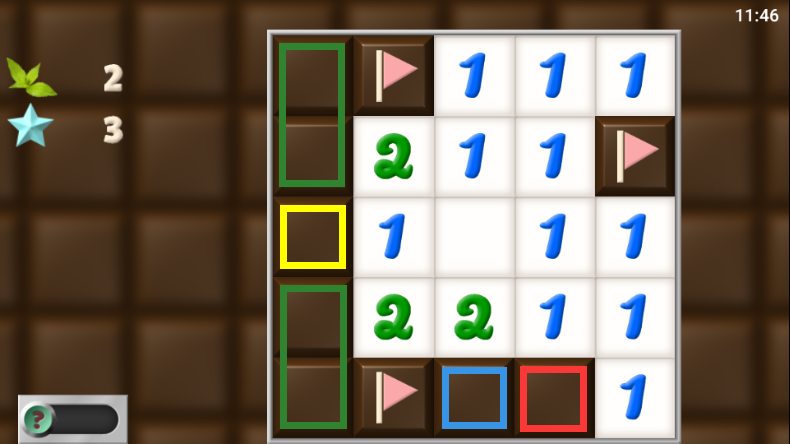
\includegraphics[width=0.7\textwidth]{puzzle/16-2.png}
\end{center}
数数,红框为雷,蓝框安全。数雷,剩下一个雷必须由左边212共用,所以黄框为雷,绿框安全。

\subsection{} % 17
\begin{center}
    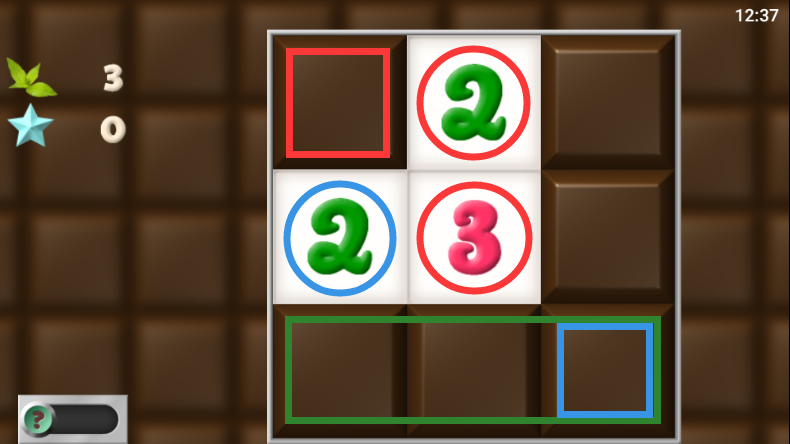
\includegraphics[width=0.7\textwidth]{puzzle/17-1.png}
\end{center}
红圈23减法得绿框有1雷;绿框再和蓝圈2做减法得红框为雷,蓝框安全。像这种用前一个减法的结论和下一个数字继续做减法的操作,我们称为连续减法。例如这里称为232连续减法。连续减法是可逆的,无论从哪边开始减,得到的结论是相同的。
\begin{center}
    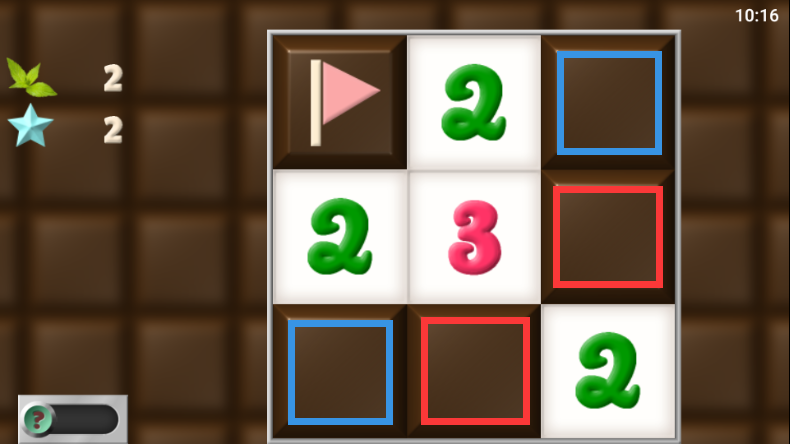
\includegraphics[width=0.7\textwidth]{puzzle/17-2.png}
\end{center}
数数,红框为雷,蓝框安全。

\subsection{} % 18
\begin{center}
    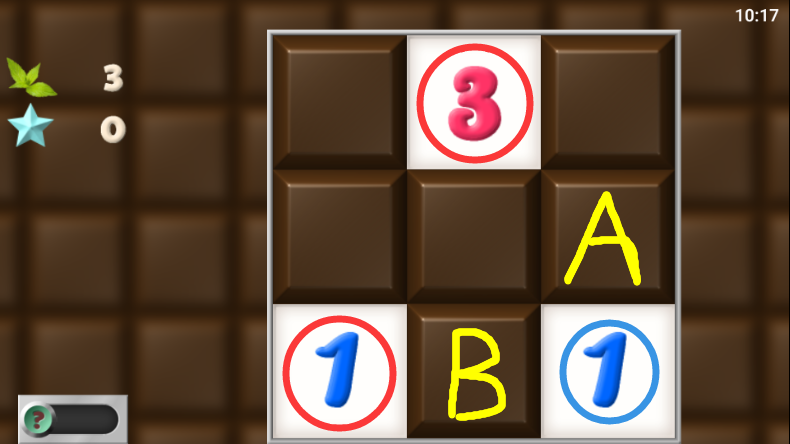
\includegraphics[width=0.7\textwidth]{puzzle/18-1.png}
\end{center}
红圈13减法得$A\ge B$,又因为蓝圈1,$B$安全。
\begin{center}
    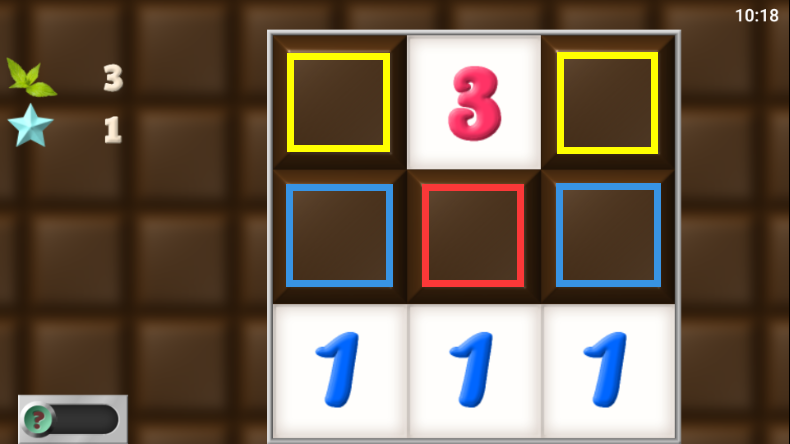
\includegraphics[width=0.7\textwidth]{puzzle/18-2.png}
\end{center}
111定式,红框为雷,蓝框安全。数数,黄框为雷。

\subsection{} % 19
\begin{center}
    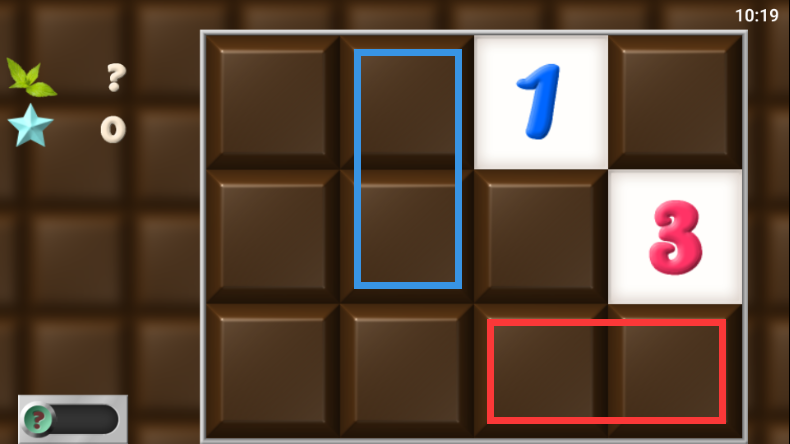
\includegraphics[width=0.7\textwidth]{puzzle/19-1.png}
\end{center}
红圈13减法得红框为雷,蓝框安全。
\begin{center}
    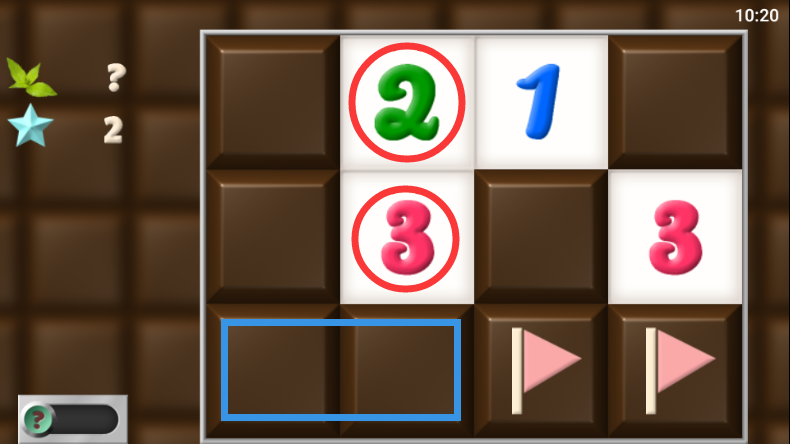
\includegraphics[width=0.7\textwidth]{puzzle/19-2.png}
\end{center}
红圈23减法得蓝框安全。
\begin{center}
    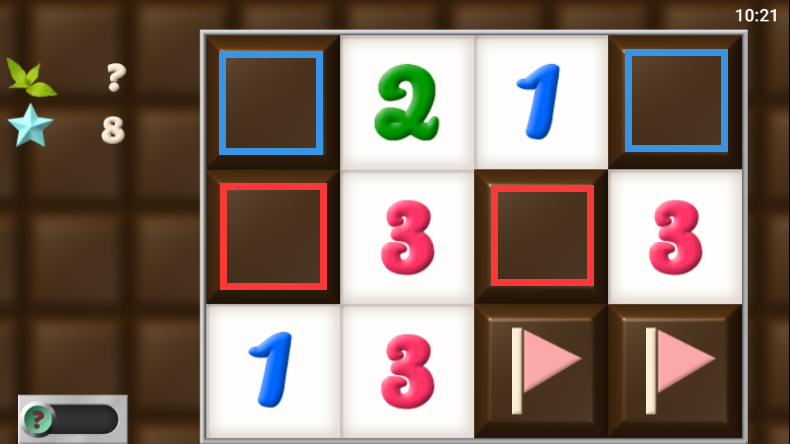
\includegraphics[width=0.7\textwidth]{puzzle/19-3.png}
\end{center}
数数,红框为雷,蓝框安全。

\subsection{} % 20
\begin{center}
    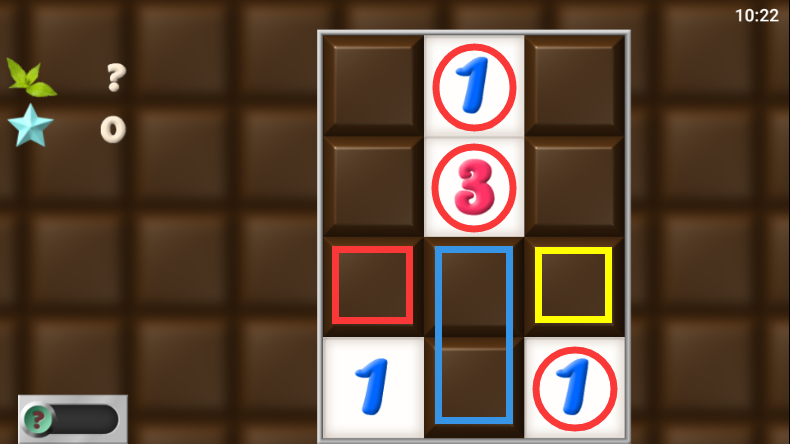
\includegraphics[width=0.7\textwidth]{puzzle/20-1.png}
\end{center}
红圈131连续减法得红框为雷,同理黄框为雷。数数,蓝框安全。

\subsection{} % 21
\begin{center}
    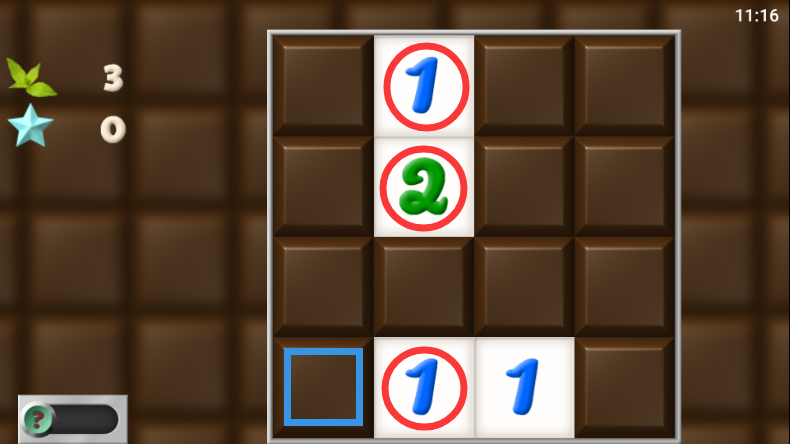
\includegraphics[width=0.7\textwidth]{puzzle/21-1.png}
\end{center}
红圈121连续减法得蓝框安全。
\begin{center}
    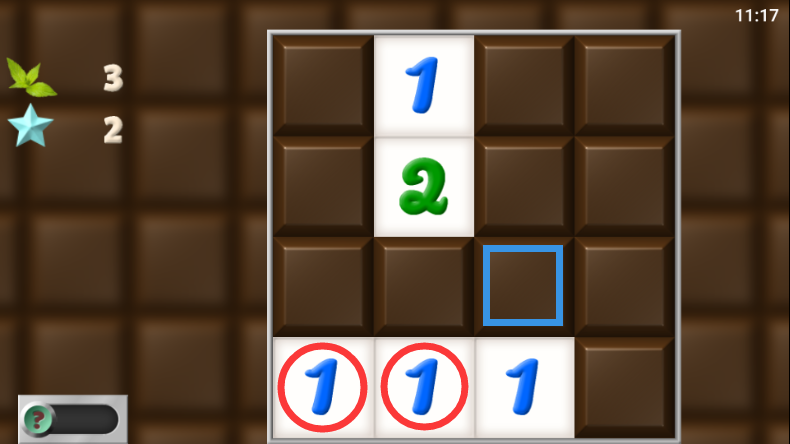
\includegraphics[width=0.7\textwidth]{puzzle/21-2.png}
\end{center}
红圈11减法得蓝框安全。
\begin{center}
    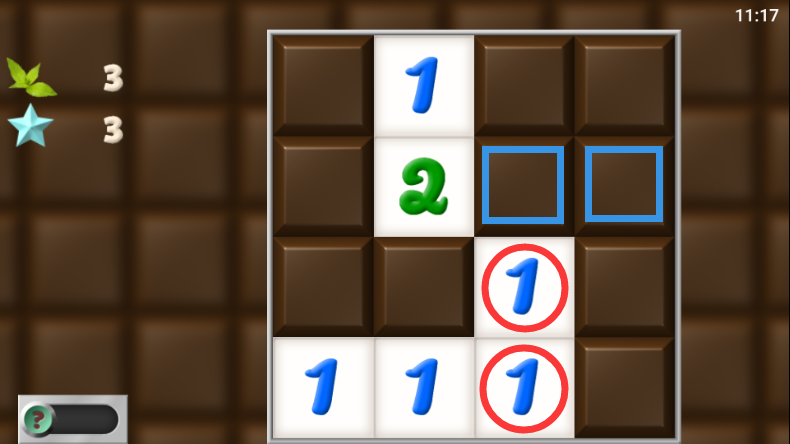
\includegraphics[width=0.7\textwidth]{puzzle/21-3.png}
\end{center}
红圈11减法得蓝框安全。
\begin{center}
    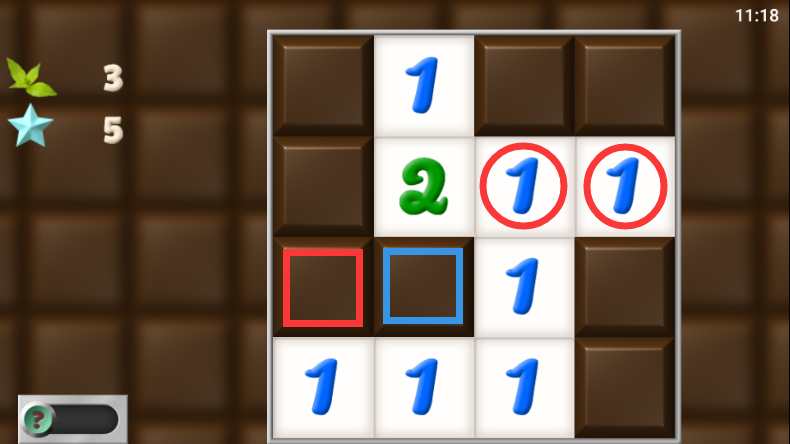
\includegraphics[width=0.7\textwidth]{puzzle/21-4.png}
\end{center}
红圈11减法得蓝框安全。数数,红框为雷。
\begin{center}
    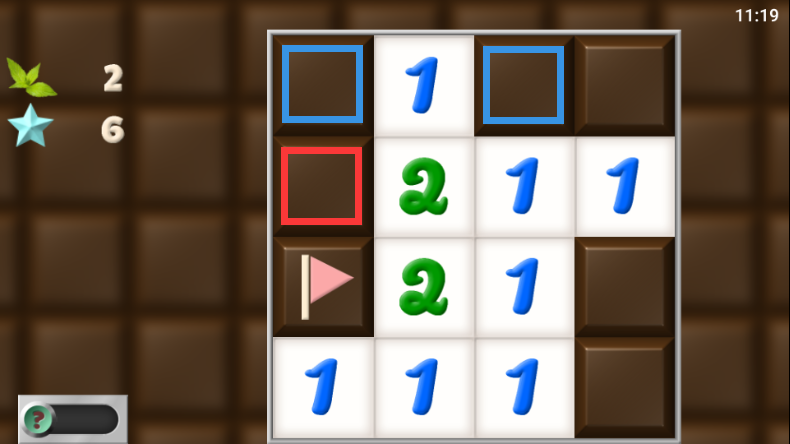
\includegraphics[width=0.7\textwidth]{puzzle/21-5.png}
\end{center}
数数,红框为雷,蓝框安全。
\begin{center}
    \includegraphics[width=0.7\textwidth]{puzzle/21-6.png}
\end{center}
数数,红框为雷,蓝框安全。

\subsection{} % 22
\begin{center}
    \includegraphics[width=0.7\textwidth]{puzzle/22-1.png}
\end{center}
红圈22减法得蓝框安全。
\begin{center}
    \includegraphics[width=0.7\textwidth]{puzzle/22-2.png}
\end{center}
红圈2321连续减法得红框为雷,蓝框安全。
\begin{center}
    \includegraphics[width=0.7\textwidth]{puzzle/22-3.png}
\end{center}
数数,红框为雷。数雷,两个绿框各有1雷,蓝框安全。
\begin{center}
    \includegraphics[width=0.7\textwidth]{puzzle/22-4.png}
\end{center}
数数,红框为雷,蓝框安全。

\subsection{} % 23
\begin{center}
    \includegraphics[width=0.7\textwidth]{puzzle/23-1.png}
\end{center}
红圈13减法得红框为雷。再用蓝圈1231连续减法得蓝框安全。
\begin{center}
    \includegraphics[width=0.7\textwidth]{puzzle/23-2.png}
\end{center}
数数,红框为雷,蓝框安全。
\begin{center}
    \includegraphics[width=0.7\textwidth]{puzzle/23-3.png}
\end{center}
数数,红框为雷,蓝框安全。

\subsection{} % 24
\begin{center}
    \includegraphics[width=0.7\textwidth]{puzzle/24-1.png}
\end{center}
两绿框各有1雷,再用红圈32减法得红框为雷,蓝框安全。
\begin{center}
    \includegraphics[width=0.7\textwidth]{puzzle/24-2.png}
\end{center}
数数,红框为雷,蓝框安全。

\subsection{} % 25
\begin{center}
    \includegraphics[width=0.7\textwidth]{puzzle/25-1.png}
\end{center}
红圈1221连续减法得蓝框安全。
\begin{center}
    \includegraphics[width=0.7\textwidth]{puzzle/25-2.png}
\end{center}
红圈121连续减法得$A=B$,又因为蓝圈1,$AB$均安全。数数,红框为雷,蓝框安全。

\subsection{} % 26
\begin{center}
    \includegraphics[width=0.7\textwidth]{puzzle/26-1.png}
\end{center}
红圈为角131定式,红框为雷,蓝框安全。数数,黄框为雷。
\begin{center}
    \includegraphics[width=0.7\textwidth]{puzzle/26-2.png}
\end{center}
数数,红框为雷,蓝框安全。

\subsection{} % 27
\begin{center}
    \includegraphics[width=0.7\textwidth]{puzzle/27-1.png}
\end{center}
红圈12减法得红框为雷,蓝框安全。
\begin{center}
    \includegraphics[width=0.7\textwidth]{puzzle/27-2.png}
\end{center}
红圈为角131定式,红框为雷。数数,蓝框安全。
\begin{center}
    \includegraphics[width=0.7\textwidth]{puzzle/27-3.png}
\end{center}
数数,红框为雷,蓝框安全。数雷,黄框为雷,绿框安全。

\subsection{} % 28
\begin{center}
    \includegraphics[width=0.7\textwidth]{puzzle/28-1.png}
\end{center}
红圈343连续减法得红框为雷。再用蓝圈232连续减法得蓝框安全。
\begin{center}
    \includegraphics[width=0.7\textwidth]{puzzle/28-2.png}
\end{center}
数数,红框为雷,蓝框安全。

\subsection{} % 29
\begin{center}
    \includegraphics[width=0.7\textwidth]{puzzle/29-1.png}
\end{center}
红圈11减法得蓝框安全。
\begin{center}
    \includegraphics[width=0.7\textwidth]{puzzle/29-2.png}
\end{center}
红圈2321连续减法得红框为雷,蓝框安全。
\begin{center}
    \includegraphics[width=0.7\textwidth]{puzzle/29-3.png}
\end{center}
红圈51减法得红框为雷。数数,蓝框安全。
\begin{center}
    \includegraphics[width=0.7\textwidth]{puzzle/29-4.png}
\end{center}
数数,红框为雷。数雷,黄框为雷,蓝框安全。

\subsection{} % 30
\begin{center}
    \includegraphics[width=0.7\textwidth]{puzzle/30-1.png}
\end{center}
红圈444连续减法得红框为雷。数数,蓝框安全。
\begin{center}
    \includegraphics[width=0.7\textwidth]{puzzle/30-2.png}
\end{center}
数数,红框为雷,蓝框安全。

\subsection{} % 31
\begin{center}
    \includegraphics[width=0.7\textwidth]{puzzle/31-1.png}
\end{center}
122连续减法得红框为雷,蓝框安全。
\begin{center}
    \includegraphics[width=0.7\textwidth]{puzzle/31-2.png}
\end{center}
红圈52减法得红框为雷,蓝框安全。数数,黄框为雷。数雷,橙框为雷,绿框安全。

\subsection{} % 32
\begin{center}
    \includegraphics[width=0.7\textwidth]{puzzle/32-1.png}
\end{center}
红圈11减法得蓝框安全。
\begin{center}
    \includegraphics[width=0.7\textwidth]{puzzle/32-2.png}
\end{center}
红圈241连续减法得红框为雷,蓝框安全。
\begin{center}
    \includegraphics[width=0.7\textwidth]{puzzle/32-3.png}
\end{center}
数数,红框为雷,蓝框安全。
\begin{center}
    \includegraphics[width=0.7\textwidth]{puzzle/32-4.png}
\end{center}
红圈24减法得红框为雷。数雷,黄框为雷,蓝框安全。

\subsection{} % 33
\begin{center}
    \includegraphics[width=0.7\textwidth]{puzzle/33-1.png}
\end{center}
红圈11减法得蓝框安全。
\begin{center}
    \includegraphics[width=0.7\textwidth]{puzzle/33-2.png}
\end{center}
红圈121连续减法得蓝框安全。再用蓝圈12减法得红框为雷。
\begin{center}
    \includegraphics[width=0.7\textwidth]{puzzle/33-3.png}
\end{center}
红圈23减法得红框为雷。数数,蓝框安全。数雷,排除掉红圈2周围的1雷,剩下的黄框全是雷。数数,绿框安全。

\subsection{} % 34
\begin{center}
    \includegraphics[width=0.7\textwidth]{puzzle/34-1.png}
\end{center}
151连续减法得红框为雷,蓝框安全。
\begin{center}
    \includegraphics[width=0.7\textwidth]{puzzle/34-2.png}
\end{center}
红圈11减法得蓝框安全。再用蓝圈12减法得红框为雷。数数,黄框为雷,绿框安全。
\begin{center}
    \includegraphics[width=0.7\textwidth]{puzzle/34-3.png}
\end{center}
数数,红框为雷,蓝框安全。

\subsection{} % 35
\begin{center}
    \includegraphics[width=0.7\textwidth]{puzzle/35-1.png}
\end{center}
红圈11减法得蓝框安全。
\begin{center}
    \includegraphics[width=0.7\textwidth]{puzzle/35-2.png}
\end{center}
红圈11减法得蓝框安全。
\begin{center}
    \includegraphics[width=0.7\textwidth]{puzzle/35-3.png}
\end{center}
红圈1231连续减法得红框为雷,蓝框安全。
\begin{center}
    \includegraphics[width=0.7\textwidth]{puzzle/35-4.png}
\end{center}
数数,红框为雷,蓝框安全。

\subsection{} % 36
\begin{center}
    \includegraphics[width=0.7\textwidth]{puzzle/36-1.png}
\end{center}
红圈1232连续减法得蓝框安全。数数,红框为雷。
\begin{center}
    \includegraphics[width=0.7\textwidth]{puzzle/36-2.png}
\end{center}
数数,红框为雷,蓝框安全。

\subsection{} % 37
\begin{center}
    \includegraphics[width=0.7\textwidth]{puzzle/37-1.png}
\end{center}
红圈3441连续减法得红框为雷,黄框有1雷。黄框再和蓝圈33做连续减法得橙框为雷,蓝框安全。数数,粉框为雷。
\begin{center}
    \includegraphics[width=0.7\textwidth]{puzzle/37-2.png}
\end{center}
数数,红框为雷,蓝框安全。

\subsection{} % 38
\begin{center}
    \includegraphics[width=0.7\textwidth]{puzzle/38-1.png}
\end{center}
红圈22减法得$A=B$,蓝圈41减法得$A+B\ge 1$,所以$AB$都为雷。再由绿圈34减法得蓝框安全。数数,红框为雷。

\subsection{} % 39
\begin{center}
    \includegraphics[width=0.7\textwidth]{puzzle/39-1.png}
\end{center}
红圈11减法得蓝框安全。
\begin{center}
    \includegraphics[width=0.7\textwidth]{puzzle/39-2.png}
\end{center}
数雷,排除掉红圈1和2周围共3雷,剩下的绿框共1雷。蓝圈12减法得黄框共1雷。绿框和黄框做减法得$A\ge B$,又因为绿圈1,$B$安全。
\begin{center}
    \includegraphics[width=0.7\textwidth]{puzzle/39-3.png}
\end{center}
数数,红框为雷,蓝框安全。

\subsection{} % 40
\begin{center}
    \includegraphics[width=0.7\textwidth]{puzzle/40-1.png}
\end{center}
红圈32减法得$A\ge B$;蓝圈121做连续减法得$A\ge C$;又因为左下角1,$B$和$C$必有一个为雷,所以$A$为雷。数数,蓝框安全。
\begin{center}
    \includegraphics[width=0.7\textwidth]{puzzle/40-2.png}
\end{center}
数数,红框为雷,蓝框安全。

\subsection{} % 41
\begin{center}
    \includegraphics[width=0.7\textwidth]{puzzle/41-1.png}
\end{center}
红圈21减法得红框为雷,蓝框安全。
\begin{center}
    \includegraphics[width=0.7\textwidth]{puzzle/41-2.png}
\end{center}
红圈121连续减法得蓝框安全。
\begin{center}
    \includegraphics[width=0.7\textwidth]{puzzle/41-3.png}
\end{center}
数雷,排除两个红圈2周围共3雷后得红框为雷。数数,蓝框安全。然后蓝圈21减法得黄框为雷。
\begin{center}
    \includegraphics[width=0.7\textwidth]{puzzle/41-4.png}
\end{center}
数数,红框为雷,蓝框安全。

\subsection{} % 42
\begin{center}
    \includegraphics[width=0.7\textwidth]{puzzle/42-1.png}
\end{center}
红圈41减法得红框为雷,蓝框安全。
\begin{center}
    \includegraphics[width=0.7\textwidth]{puzzle/42-2.png}
\end{center}
红圈131连续减法得蓝框安全。数雷,排除红圈3周围2雷后得红框为雷。数数,绿框安全。
\begin{center}
    \includegraphics[width=0.7\textwidth]{puzzle/42-3.png}
\end{center}
数数,红框为雷,蓝框安全。

\subsection{} % 43
\begin{center}
    \includegraphics[width=0.7\textwidth]{puzzle/43-1.png}
\end{center}
红圈21减法得红框为雷,蓝框安全。然后蓝圈231连续减法得绿框安全。
\begin{center}
    \includegraphics[width=0.7\textwidth]{puzzle/43-2.png}
\end{center}
红圈21减法得红框为雷。数雷,排除两个蓝圈2周围共3雷后得蓝框安全。
\begin{center}
    \includegraphics[width=0.7\textwidth]{puzzle/43-3.png}
\end{center}
数数,红框为雷,蓝框安全。

\subsection{} % 44
\begin{center}
    \includegraphics[width=0.7\textwidth]{puzzle/44-1.png}
\end{center}
红圈233连续减法得红框为雷。数数,蓝框安全。
\begin{center}
    \includegraphics[width=0.7\textwidth]{puzzle/44-2.png}
\end{center}
红圈22减法得红框为雷。蓝圈23减法得黄框为雷。数数,蓝框安全。
\begin{center}
    \includegraphics[width=0.7\textwidth]{puzzle/44-3.png}
\end{center}
数数,红框为雷,蓝框安全。

\subsection{} % 45
\begin{center}
    \includegraphics[width=0.7\textwidth]{puzzle/45-1.png}
\end{center}
两个绿框各1雷,然后32减法得红框为雷,蓝框安全。
\begin{center}
    \includegraphics[width=0.7\textwidth]{puzzle/45-2.png}
\end{center}
红圈221连续减法得蓝框安全。数数,红框为雷。
\begin{center}
    \includegraphics[width=0.7\textwidth]{puzzle/45-3.png}
\end{center}
数数,红框为雷,蓝框安全。

\subsection{} % 46
\begin{center}
    \includegraphics[width=0.7\textwidth]{puzzle/46-1.png}
\end{center}
1321连续减法得红框为雷,蓝框安全。
\begin{center}
    \includegraphics[width=0.7\textwidth]{puzzle/46-2.png}
\end{center}
红圈232连续减法得红框为雷。再用蓝圈13减法得蓝框安全。
\begin{center}
    \includegraphics[width=0.7\textwidth]{puzzle/46-3.png}
\end{center}
红圈34减法得红框为雷。数数,蓝框安全。
\begin{center}
    \includegraphics[width=0.7\textwidth]{puzzle/46-4.png}
\end{center}
数数,红框为雷,蓝框安全。

\subsection{} % 47
\begin{center}
    \includegraphics[width=0.7\textwidth]{puzzle/47-1.png}
\end{center}
四个角分别用角222定式得红框为雷。数数,蓝框安全。

\subsection{} % 48
\begin{center}
    \includegraphics[width=0.7\textwidth]{puzzle/48-1.png}
\end{center}
红圈22减法得$A\ge B$,另一边同理得$B\ge A$,所以$A=B$。回顾红圈22减法得蓝框安全,同理绿框安全。数数,红框为雷。

\subsection{} % 49
\begin{center}
    \includegraphics[width=0.7\textwidth]{puzzle/49-1.png}
\end{center}
数雷,排除4个2周围共8雷后得蓝框安全。
\begin{center}
    \includegraphics[width=0.7\textwidth]{puzzle/49-2.png}
\end{center}
数数,红框为雷,蓝框安全。

\subsection{} % 50
\begin{center}
    \includegraphics[width=0.7\textwidth]{puzzle/50-1.png}
\end{center}
红圈123连续减法得红框为雷,蓝框安全。再用蓝圈32减法得黄框为雷。
\begin{center}
    \includegraphics[width=0.7\textwidth]{puzzle/50-2.png}
\end{center}
红圈223连续减法得红框为雷,蓝框安全。
\begin{center}
    \includegraphics[width=0.7\textwidth]{puzzle/50-3.png}
\end{center}
数数,红框为雷,蓝框安全。

\subsection{} % 51
\begin{center}
    \includegraphics[width=0.7\textwidth]{puzzle/51-1.png}
\end{center}
红圈1221连续减法得蓝框安全。
\begin{center}
    \includegraphics[width=0.7\textwidth]{puzzle/51-2.png}
\end{center}
红圈121连续减法得蓝框安全。数数,红框为雷。
\begin{center}
    \includegraphics[width=0.7\textwidth]{puzzle/51-3.png}
\end{center}
数数,红框为雷,蓝框安全。

\subsection{} % 52
\begin{center}
    \includegraphics[width=0.7\textwidth]{puzzle/52-1.png}
\end{center}
红圈22减法得$A\ge B$,$A\ge C$;蓝圈22减法得$C\ge D$;所以$A\ge D$。又因为绿圈4,$A+B+D\ge 1$,所以$A$为雷,同理红框为雷。再用橙圈222连续减法得橙框为雷,同理$C$为雷。
\begin{center}
    \includegraphics[width=0.7\textwidth]{puzzle/52-2.png}
\end{center}
数数,红框为雷,蓝框安全。

\subsection{} % 53
\begin{center}
    \includegraphics[width=0.7\textwidth]{puzzle/53-1.png}
\end{center}
数数,红框为雷。再用红圈242连续减法得黄框为雷。再用蓝圈32减法得橙框为雷,蓝框安全。
\begin{center}
    \includegraphics[width=0.7\textwidth]{puzzle/53-2.png}
\end{center}
数数,红框为雷,蓝框安全。

\subsection{} % 54
\begin{center}
    \includegraphics[width=0.7\textwidth]{puzzle/54-1.png}
\end{center}
红圈22减法得$A=B$。再用蓝圈43减法得红框为雷,蓝框安全。
\begin{center}
    \includegraphics[width=0.7\textwidth]{puzzle/54-2.png}
\end{center}
数数,红框为雷。再用红圈42减法得黄框为雷。再用蓝圈22减法得橙框为雷,蓝框安全。再用绿圈23减法得绿框安全。
\begin{center}
    \includegraphics[width=0.7\textwidth]{puzzle/54-3.png}
\end{center}
数数,红框为雷,蓝框安全。数雷,黄框为雷,绿框安全。

\subsection{} % 55
\begin{center}
    \includegraphics[width=0.7\textwidth]{puzzle/55-1.png}
\end{center}
红圈122连续减法得红框为雷。再用蓝圈243连续减法得蓝框安全。
\begin{center}
    \includegraphics[width=0.7\textwidth]{puzzle/55-2.png}
\end{center}
红圈13减法得红框为雷。数数,蓝框安全。
\begin{center}
    \includegraphics[width=0.7\textwidth]{puzzle/55-3.png}
\end{center}
数数,红框为雷,蓝框安全。
\begin{center}
    \includegraphics[width=0.7\textwidth]{puzzle/55-4.png}
\end{center}
数数,红框为雷,蓝框安全。

\subsection{} % 56
\begin{center}
    \includegraphics[width=0.7\textwidth]{puzzle/56-1.png}
\end{center}
红圈122连续减法得红框为雷。再用蓝圈122连续减法得蓝框安全。
\begin{center}
    \includegraphics[width=0.7\textwidth]{puzzle/56-2.png}
\end{center}
红圈12减法得蓝框安全。数数,红框为雷。
\begin{center}
    \includegraphics[width=0.7\textwidth]{puzzle/56-3.png}
\end{center}
数数,红框为雷,蓝框安全。

\subsection{} % 57
\begin{center}
    \includegraphics[width=0.7\textwidth]{puzzle/57-1.png}
\end{center}
红圈122连续减法得红框为雷。再用蓝圈122连续减法得蓝框安全。数数,黄框为雷。

\subsection{} % 58
\begin{center}
    \includegraphics[width=0.7\textwidth]{puzzle/58-1.png}
\end{center}
红圈22减法得$A=B$。再用蓝圈52减法得红框为雷。数数,蓝框安全。
\begin{center}
    \includegraphics[width=0.7\textwidth]{puzzle/58-2.png}
\end{center}
数雷,排除掉5周围共2雷后得红框为雷。数数,黄框为雷,蓝框安全。

\subsection{} % 59
\begin{center}
    \includegraphics[width=0.7\textwidth]{puzzle/59-1.png}
\end{center}
红圈122连续减法得$A\ge B$。又因为蓝圈1,$B$安全。
\begin{center}
    \includegraphics[width=0.7\textwidth]{puzzle/59-2.png}
\end{center}
红圈12减法得红框为雷。数数,黄框为雷,蓝框安全。

\subsection{} % 60
\begin{center}
    \includegraphics[width=0.7\textwidth]{puzzle/60-1.png}
\end{center}
红圈22减法得$A=B$,又因为绿圈3,$A+B\ge 1$,所以$AB$都是雷。蓝圈23减法得$C\ge D$,又因为绿圈3,$C+D=1$,所以$C$为雷,$D$安全。数数,红框为雷,蓝框安全。

\subsection{} % 61
\begin{center}
    \includegraphics[width=0.7\textwidth]{puzzle/61-1.png}
\end{center}
红圈11减法得$A\ge B$,又因为蓝圈1,$A+B\le 1$,所以$B$安全。
\begin{center}
    \includegraphics[width=0.7\textwidth]{puzzle/61-2.png}
\end{center}
红圈21减法得红框为雷。数数,黄框为雷,蓝框安全。

\subsection{} % 62
\begin{center}
    \includegraphics[width=0.7\textwidth]{puzzle/62-1.png}
\end{center}
红圈21减法得红框为雷,蓝框安全。数数,黄框为雷。蓝圈232形成角131定式,橙框为雷,绿框安全。

\subsection{} % 63
\begin{center}
    \includegraphics[width=0.7\textwidth]{puzzle/63-1.png}
\end{center}
红圈22减法得$A\ge B$,蓝圈21减法得$B\ge C$,所以$A\ge C$。又因为绿圈23减法得$A+C=1$,所以$A$为雷,$C$安全。
\begin{center}
    \includegraphics[width=0.7\textwidth]{puzzle/63-2.png}
\end{center}
红圈11减法得蓝框安全。数数,红框为雷,绿框安全。

\subsection{} % 64
\begin{center}
    \includegraphics[width=0.7\textwidth]{puzzle/64-1.png}
\end{center}
数雷,排除掉红圈12周围共3雷后得红框为雷。数数,蓝框安全。再用蓝圈322连续减法得黄框为雷。数数,绿框安全。
\begin{center}
    \includegraphics[width=0.7\textwidth]{puzzle/64-2.png}
\end{center}
数数,红框为雷,蓝框安全。

\subsection{} % 65
\begin{center}
    \includegraphics[width=0.7\textwidth]{puzzle/65-1.png}
\end{center}
红圈1231连续减法得红框为雷,蓝框安全。
\begin{center}
    \includegraphics[width=0.7\textwidth]{puzzle/65-2.png}
\end{center}
数雷,排除掉红圈13周围共3雷后得红框为雷。数数,黄框为雷,蓝框安全。

\subsection{} % 66
\begin{center}
    \includegraphics[width=0.7\textwidth]{puzzle/66-1.png}
\end{center}
红圈21减法得红框为雷,蓝框安全。
\begin{center}
    \includegraphics[width=0.7\textwidth]{puzzle/66-2.png}
\end{center}
数雷,排除红圈12周围共3雷后得绿框共1雷。绿框再和蓝圈1做减法得$A=B$。又因为绿圈2,$A+B\le 1$,所以$AB$均安全。数数,红框为雷。
\begin{center}
    \includegraphics[width=0.7\textwidth]{puzzle/66-3.png}
\end{center}
数数,红框为雷。红圈12减法得蓝框安全。数数,黄框为雷。

\subsection{} % 67
\begin{center}
    \includegraphics[width=0.7\textwidth]{puzzle/67-1.png}
\end{center}
红圈11减法得$A\ge B$,蓝圈22减法得$B\ge C$,所以$A\ge C$。又由于绿圈12减法得$A+C\le 1$,所以$C$安全。再用红圈11减法得$A\ge E$,橙圈22减法得$D\ge E$,绿圈12减法得$A+D=1$,所以$E$安全。
\begin{center}
    \includegraphics[width=0.7\textwidth]{puzzle/67-2.png}
\end{center}
数数,红框为雷,蓝框安全。

\subsection{} % 68
\begin{center}
    \includegraphics[width=0.7\textwidth]{puzzle/68-1.png}
\end{center}
红圈1232连续减法得蓝框安全。
\begin{center}
    \includegraphics[width=0.7\textwidth]{puzzle/68-2.png}
\end{center}
红圈11减法得$A=B$,蓝圈13减法得$A+B\ge 1$,所以$AB$均为雷。数数,红框为雷,蓝框安全。

\subsection{} % 69
\begin{center}
    \includegraphics[width=0.7\textwidth]{puzzle/69-1.png}
\end{center}
红圈11减法得$A\ge B$,蓝圈12减法得$A+B\le 1$,所以$B$安全。
\begin{center}
    \includegraphics[width=0.7\textwidth]{puzzle/69-2.png}
\end{center}
红圈22减法得蓝框安全。数数,红框为雷。蓝圈11减法得绿框安全。

\subsection{} % 70
\begin{center}
    \includegraphics[width=0.7\textwidth]{puzzle/70-1.png}
\end{center}
红圈22减法得$A=B$,再用蓝圈33减法得$C=D$,又因为绿圈2,$C+D\ge 1$,所以$CD$为雷。数数,红框为雷,$AB$为雷,蓝框安全。

\subsection{} % 71
\begin{center}
    \includegraphics[width=0.7\textwidth]{puzzle/71-1.png}
\end{center}
红圈2321连续减法得蓝框安全。
\begin{center}
    \includegraphics[width=0.7\textwidth]{puzzle/71-2.png}
\end{center}
数数,红框为雷,蓝框安全。

\subsection{} % 72
\begin{center}
    \includegraphics[width=0.7\textwidth]{puzzle/72-1.png}
\end{center}
红圈12减法得$A\ge B$,又因为蓝圈1,$A+B\le 1$,所以$B$安全。
\begin{center}
    \includegraphics[width=0.7\textwidth]{puzzle/72-2.png}
\end{center}
红圈11减法得$A\ge B$,蓝圈12减法得$B\ge C$,所以$A\ge C$。又因为绿圈1,$A+C\le 1$,所以$C$安全。
\begin{center}
    \includegraphics[width=0.7\textwidth]{puzzle/72-3.png}
\end{center}
红圈11减法得蓝框安全。
\begin{center}
    \includegraphics[width=0.7\textwidth]{puzzle/72-4.png}
\end{center}
数数,红框为雷,蓝框安全。
\begin{center}
    \includegraphics[width=0.7\textwidth]{puzzle/72-5.png}
\end{center}
数数,红框为雷,蓝框安全。

\subsection{} % 73
\begin{center}
    \includegraphics[width=0.7\textwidth]{puzzle/73-1.png}
\end{center}
红圈121连续减法得蓝框安全。
\begin{center}
    \includegraphics[width=0.7\textwidth]{puzzle/73-2.png}
\end{center}
红圈122连续减法得绿框有1雷。数雷,排除掉绿框和蓝圈2共3雷后得红框为雷。绿圈12减法得蓝框安全。
\begin{center}
    \includegraphics[width=0.7\textwidth]{puzzle/73-3.png}
\end{center}
红圈23减法得红框为雷。数数,黄框为雷,蓝框安全。

\subsection{} % 74
\begin{center}
    \includegraphics[width=0.7\textwidth]{puzzle/74-1.png}
\end{center}
红圈131连续减法得$A\ge B$,又因为蓝圈1,$A+B\le 1$,所以$B$安全。
\begin{center}
    \includegraphics[width=0.7\textwidth]{puzzle/74-2.png}
\end{center}
红圈121定式得红框为雷,蓝框安全。蓝圈21减法得$A\ge B$,又因为绿圈3,$A+B\le 1$,所以$B$安全。
\begin{center}
    \includegraphics[width=0.7\textwidth]{puzzle/74-3.png}
\end{center}
红圈132定式得红框为雷,蓝框安全。

\subsection{} % 75
\begin{center}
    \includegraphics[width=0.7\textwidth]{puzzle/75-1.png}
\end{center}
红圈13定式得红框为雷。蓝圈12减法得$A\ge B$,又由绿圈13减法得$A+B\le 1$,所以$B$安全。
\begin{center}
    \includegraphics[width=0.7\textwidth]{puzzle/75-2.png}
\end{center}
数数,红框为雷,蓝框安全。

\subsection{} % 76
\begin{center}
    \includegraphics[width=0.7\textwidth]{puzzle/76-1.png}
\end{center}
红圈14减法得$A\ge B+C$,蓝圈22减法得$D=A$,所以$D\ge B+C$。又因为红圈1,$B+C+D\le 1$,所以$BC$均安全。数数,红框为雷,$AD$为雷,蓝框安全。
\begin{center}
    \includegraphics[width=0.7\textwidth]{puzzle/76-2.png}
\end{center}
数数,红框为雷,蓝框安全。

\subsection{} % 77
\begin{center}
    \includegraphics[width=0.7\textwidth]{puzzle/77-1.png}
\end{center}
红圈12减法得$A\ge D$,$B\ge D$,蓝圈13减法得$C\ge D$,又因为绿圈2,$A+B+C\le 2$,所以$D$安全。
\begin{center}
    \includegraphics[width=0.7\textwidth]{puzzle/77-2.png}
\end{center}
红圈11减法得蓝框安全。
\begin{center}
    \includegraphics[width=0.7\textwidth]{puzzle/77-3.png}
\end{center}
红圈23减法得红框为雷,蓝框安全。
\begin{center}
    \includegraphics[width=0.7\textwidth]{puzzle/77-4.png}
\end{center}
数数,红框为雷,蓝框安全。

\subsection{} % 78
\begin{center}
    \includegraphics[width=0.7\textwidth]{puzzle/78-1.png}
\end{center}
红圈12减法得$A\ge B$,蓝圈12减法得$C\ge B$,又因为绿圈1,$A+C\le 1$,所以$B$安全。再用红圈12和橙圈1做连续减法得$A\ge D$,蓝圈12减法得$C\ge D$,回顾$A+C\le 1$,$D$安全。
\begin{center}
    \includegraphics[width=0.7\textwidth]{puzzle/78-2.png}
\end{center}
红圈22减法得蓝框安全。再用蓝圈21减法得红框为雷,绿框安全。数数,橙框为雷,黄框安全。

\subsection{} % 79
\begin{center}
    \includegraphics[width=0.7\textwidth]{puzzle/79-1.png}
\end{center}
1241连续减法得红框为雷,蓝框安全。
\begin{center}
    \includegraphics[width=0.7\textwidth]{puzzle/79-2.png}
\end{center}
红圈222连续减法得蓝框安全。
\begin{center}
    \includegraphics[width=0.7\textwidth]{puzzle/79-3.png}
\end{center}
数数,红框为雷,蓝框安全。

\subsection{} % 80
\begin{center}
    \includegraphics[width=0.7\textwidth]{puzzle/80-1.png}
\end{center}
红圈121定式得蓝框安全。
\begin{center}
    \includegraphics[width=0.7\textwidth]{puzzle/80-2.png}
\end{center}
红圈11减法得$A=B$,又由蓝圈122减法得$A+B\le 1$,所以$AB$均安全。再用蓝圈122减法得红框为雷。数数,蓝框安全。
\begin{center}
    \includegraphics[width=0.7\textwidth]{puzzle/80-3.png}
\end{center}
数数,红框为雷,蓝框安全。

\subsection{} % 81
\begin{center}
    \includegraphics[width=0.7\textwidth]{puzzle/81-1.png}
\end{center}
红圈13减法得$A+B+C\ge D+1$,蓝圈1得$C\le 1-D$,所以$A+B\ge 2D$。又因为绿圈1,$A+B\le 1$,所以$D$安全。
\begin{center}
    \includegraphics[width=0.7\textwidth]{puzzle/81-2.png}
\end{center}
红圈11减法得$A=B$,再用蓝圈131连续减法得红框为雷,蓝框安全。
\begin{center}
    \includegraphics[width=0.7\textwidth]{puzzle/81-3.png}
\end{center}
红圈12减法得蓝框安全。
\begin{center}
    \includegraphics[width=0.7\textwidth]{puzzle/81-4.png}
\end{center}
数数,红框为雷,蓝框安全。

\subsection{} % 82
\begin{center}
    \includegraphics[width=0.7\textwidth]{puzzle/82-1.png}
\end{center}
红圈11减法得$A=B$,又由蓝圈122减法得$A+B\le 1$,所以$AB$均安全。
\begin{center}
    \includegraphics[width=0.7\textwidth]{puzzle/82-2.png}
\end{center}
红圈11减法得蓝框安全。数数,红框为雷,绿框安全。

\subsection{} % 83
\begin{center}
    \includegraphics[width=0.7\textwidth]{puzzle/83-1.png}
\end{center}
红圈222连续减法得红框为雷,蓝框安全。
\begin{center}
    \includegraphics[width=0.7\textwidth]{puzzle/83-2.png}
\end{center}
红圈35减法得红框为雷。数数,蓝框安全。数雷,黄框为雷,绿框安全。

\subsection{} % 84
\begin{center}
    \includegraphics[width=0.7\textwidth]{puzzle/84-1.png}
\end{center}
红圈22减法得$A\ge B$,蓝圈21减法得$B\ge C$,绿圈22减法得$A=D$,所以$D\ge C$。又因为蓝圈1,$D+C\le 1$,所以$C$安全。
\begin{center}
    \includegraphics[width=0.7\textwidth]{puzzle/84-2.png}
\end{center}
红圈12减法得红框为雷。再用蓝圈222连续减法得黄框为雷。再用绿圈122连续减法得蓝框安全。
\begin{center}
    \includegraphics[width=0.7\textwidth]{puzzle/84-3.png}
\end{center}
数数,红框为雷,蓝框安全。

\subsection{} % 85
\begin{center}
    \includegraphics[width=0.7\textwidth]{puzzle/85-1.png}
\end{center}
红圈12减法得$A\ge B$,又由蓝圈12减法得$A+B\le 1$,所以$B$安全。
\begin{center}
    \includegraphics[width=0.7\textwidth]{puzzle/85-2.png}
\end{center}
红圈12减法得$A\ge B$,蓝圈121连续减法得$C\ge A$,所以$C\ge B$。又因为红圈1,$B+C\le 1$,所以$B$安全。
\begin{center}
    \includegraphics[width=0.7\textwidth]{puzzle/85-3.png}
\end{center}
红圈11减法得蓝框安全。
\begin{center}
    \includegraphics[width=0.7\textwidth]{puzzle/85-4.png}
\end{center}
红圈11减法得蓝框安全。数数,红框为雷。蓝圈12减法得黄框为雷。
\begin{center}
    \includegraphics[width=0.7\textwidth]{puzzle/85-5.png}
\end{center}
数数,红框为雷,蓝框安全。

\subsection{} % 86
\begin{center}
    \includegraphics[width=0.7\textwidth]{puzzle/86-1.png}
\end{center}
红圈121连续减法得蓝框安全。
\begin{center}
    \includegraphics[width=0.7\textwidth]{puzzle/86-2.png}
\end{center}
红圈532连续减法得红框为雷,蓝框安全。数数,绿框安全。数雷,橙框为雷,黄框安全。

\subsection{} % 87
\begin{center}
    \includegraphics[width=0.7\textwidth]{puzzle/87-1.png}
\end{center}
红圈11减法得蓝框安全。
\begin{center}
    \includegraphics[width=0.7\textwidth]{puzzle/87-2.png}
\end{center}
红圈11减法得$A\ge B$,又由蓝圈12减法得$A+B\le 1$,所以$B$安全。再用绿圈12减法得红框为雷。数数,蓝框安全。再用橙圈11减法得绿框安全。
\begin{center}
    \includegraphics[width=0.7\textwidth]{puzzle/87-3.png}
\end{center}
数数,红框为雷,蓝框安全。

\subsection{} % 88
\begin{center}
    \includegraphics[width=0.7\textwidth]{puzzle/88-1.png}
\end{center}
红圈121连续减法得蓝框安全。再用蓝圈22减法得$A=B$,又由绿圈15减法得$A+B\ge 1$,所以$AB$均为雷。数数,绿框安全。
\begin{center}
    \includegraphics[width=0.7\textwidth]{puzzle/88-2.png}
\end{center}
数数,红框为雷,蓝框安全。
\begin{center}
    \includegraphics[width=0.7\textwidth]{puzzle/88-3.png}
\end{center}
数数,红框为雷,蓝框安全。

\subsection{} % 89
\begin{center}
    \includegraphics[width=0.7\textwidth]{puzzle/89-1.png}
\end{center}
红圈13减法得$A+B\ge C+1$,蓝圈12减法得$A+B\le D+1$,所以$D\ge C$。又由红圈13减法得$A\ge C$,由绿圈2得$A+C+D\le 2$,所以$C$安全。
\begin{center}
    \includegraphics[width=0.7\textwidth]{puzzle/89-2.png}
\end{center}
红圈12减法得红框为雷。数雷,排除掉蓝圈13周围共3雷后知黄框为雷。数数,橙框为雷,蓝框安全。